\section{Teoria}
\label{aGabor_teoria}
Filtr w grafice komputerowej jest tak zwaną konwolucją dyskretną \cite{Tadeusiewicz} obrazu. Dla przypadku 2 wymiarów będzie ona przedstawiona poniżej.
$$
	L'(m, n) = (w \times L)(m, n) = \sum_{i, j \in K}L(m-i, n-j)w(i, j)	
$$
Należy wyjaśnić, że w powyższym przykładzie $L$ jest obrazem początkowym, gdzie $L(x, y)$ jest punktem w tym obrazie określonym współrzędnymi $x$ i $y$. Natomiast $w(x, y)$ jest filtrem, którego składowe $x$ i $y$ są tak samo interpretowane. Wynikiem przedstawionej w ten sposób filtracji obrazu jest $L'$.\\
Można powiedzieć, że przy filtrowaniu posiadamy 3 macierze/tablice(2D) różnych rozmiarów. Z czego przyjmuje się, że macierze $L$ i $L'$ są tych samych rozmiarów, a macierz $w$ jest innych rozmiarów (najlepiej aby jej rozmiary przedstawiane były za pomocą 2 liczb nieparzystych) i jest dużo mniejsza od $L$. Macierz $w$ jest ,,oknem filtru''s.\\

Filtrowanie jest procesem w którym dla każdego piksela z obrazu wejściowego -- nawiązując do oznaczeń zaproponowanych powyżej -- $L$ kolor odpowiadającego mu piksla w obrazie wyjściowym ($L'$) jest zależny od ważonej sumy wartości koloru piksli go otaczających. Wagi dla tego przekształcenia są określone przez okno filtru i przyjmuje się, że środkowemu punktowi okna filtru odpowiada wybrany wcześniej piksel w obrazie $L$. Dodatkowo wymaga się, aby zostały określone warunki na podstawie których będzie można to przekształcenie stosować na krawędziach obrazu, dochodzi tam bowiem do sytuacji, w których okno filtru wykracza poza obraz. Przyjmuje się, że w takich wypadkach nieistniejące piksle nie biorą udziału w wyliczeniach wartości koloru dla danego piksla leżącego przy krawędzi. Należy jednak dodatkowo zwrócić uwagę na fakt, że obraz jest dwuwymiarową tablicą kolorów, z których każdy jest w określonych granicach. Wymagane jest więc, aby po przekształceniu obrazu danym filtrem doprowadzić jego wartości kolorów w taki sposób, aby mógł on odzwierciedlać obraz.\\

Przykładowo obraz może być dwuwymiarową tablicą piksli, z których każdy jest określonego koloru, a kolor ten jest przedstawiony np. jako wartość jasności (dla obrazów czarno-białych) i mieści się w zakresie $(0, 255)$. Po przekształceniu filtrem o oknie wielkości $3\times3$, w którym wartości są z zakresu $(-1, 1)$ należałoby wartości w obrazie wynikowym tak przemnożyć, aby również przedstawiały określony wcześniej zakres. 

\subsection{Funkcja Gabora}
\label{aGabor_funkcja}

Funkcja Gabora \cite{Movellan}, która jest głównym składnikiem filtru Gabora jest bardzo prostym złożeniem dwóch, tak naprawdę elementarnych funkcji. Jako złożenie funkcji autor ma na myśli prosty iloczyn -- jak to jest przedstawione we wzorze \ref{eqn:aGabor_wzor1}.
\begin{align}\label{eqn:aGabor_wzor1}
g(x, y) = s(x, y) w_r (x, y)
\end{align}
W przedstawionym powyżej wzorze należy wyszczególnić dwa elementy: 
\begin{description}
\item [$s(x, y)$] -- jest zespoloną sinusoidą, nazywaną nośnikiem\footnote{Z języka angielskiego carrier.}
\item [$w_r (x, y)$] -- jest dwuwymiarową funkcją o kształcie funkcji Gaussa, nazywaną powłoką\footnote{Z języka angielskiego envelope.}
\end{description}

\subsubsection{Nośnik}
\label{aGabor_carrier}

Zespolona sinusoida jest odwzorowaniem funkcji \ref{eqn:aGabor_c_sinus} na płaszczyźnie.
\begin{align}\label{eqn:aGabor_c_sinus}
s(x, y) = exp(j(2\pi(u_0x + v_0y)+P))
\end{align}
W podanym wyżej wzorze można wydzielić parametry:
\begin{description}
\item [$P$] -- faza sinusoidy
\item [$(u_0, v_0)$] -- wektor, który opisuje częstotliwość przestrzenną sinusoidy\footnote{Z języka angielskiego spatial frequency.}
\end{description}

Modelowanie funkcji Gabora bardzo wygodnie jest przedstawiać jako złożenie części urojonej i rzeczywistej, tak jak to jest zobrazowane we wzorach \ref{eqn:aGabor_re} i \ref{eqn:aGabor_im}.
\begin{align}\label{eqn:aGabor_re}
\Re(s(x, y)) = \cos(2\pi(u_0x + v_0y)+P)\\
\label{eqn:aGabor_im}
\Im(s(x, y)) = \sin(2\pi(u_0x + v_0y)+P)
\end{align}

Chcąc przekształcić tak przedstawioną funkcję do współrzędnych biegunowych -- co w efekcie dużo uprości -- wymagane jest zastosowanie kilku przekształceń, które bezpośrednio wynikają z zastosowania kilku reguł matematycznych.

\begin{align}\label{eqn:aGabor_F0}
F_0 = \sqrt{u_0^2 + v_0^2}\\
\label{eqn:aGabor_w0}
\omega_0 = \tan^{-1} \Big(  \frac{v_0}{u_0}\Big)
\end{align}
Gdzie: 
\begin{description}
\item [$F_0$] -- wzmocnienie\footnote{Z języka angielskiego magnitude.}
\item [$\omega_0$] -- kierunek
\end{description}

Rzecz jasna można odwrócić sytuację i przedstawić $u_0$ i $v_0$ jako funkcję $F_0$ i $\omega_0$, jak to jest przedstawione we wzorach \ref{eqn:aGabor_u0} i \ref{eqn:aGabor_v0}.

\begin{align}\label{eqn:aGabor_u0}
u_0 = F_0 \cos\omega_0\\
\label{eqn:aGabor_v0}
v_0 = F_0 \sin\omega_0
\end{align}

W tej reprezentacji funkcja ma następującą postać.

\begin{align}\label{eqn:aGabor_polar}
s(x, y) = exp(j(2\pi F_0(x\cos\omega_0 + y\sin\omega_0)+P))
\end{align}

Co podczas implementacji najprościej przedstawić jako następującą funkcję.

\begin{align}\label{eqn:aGabor_implementacja}
s(x, y) = sin(2\pi F_0(x\cos\omega_0 + y\sin\omega_0)+P)
\end{align}

Takie przedstawienie nośnika czyni z niego jakby funkcję sinus w przestrzeni, która jest rozciągnięta w tym trzecim wymiarze. Trochę przypomina płaską falę na wodzie, co obrazuje dobrze rysunek \ref{fig:aGabor_carrier}.\\
Sterując teraz wartością $\omega_0$ można obracać funkcję wokół punktu $(0, 0)$.

\begin{figure}[ht]
	\centering
	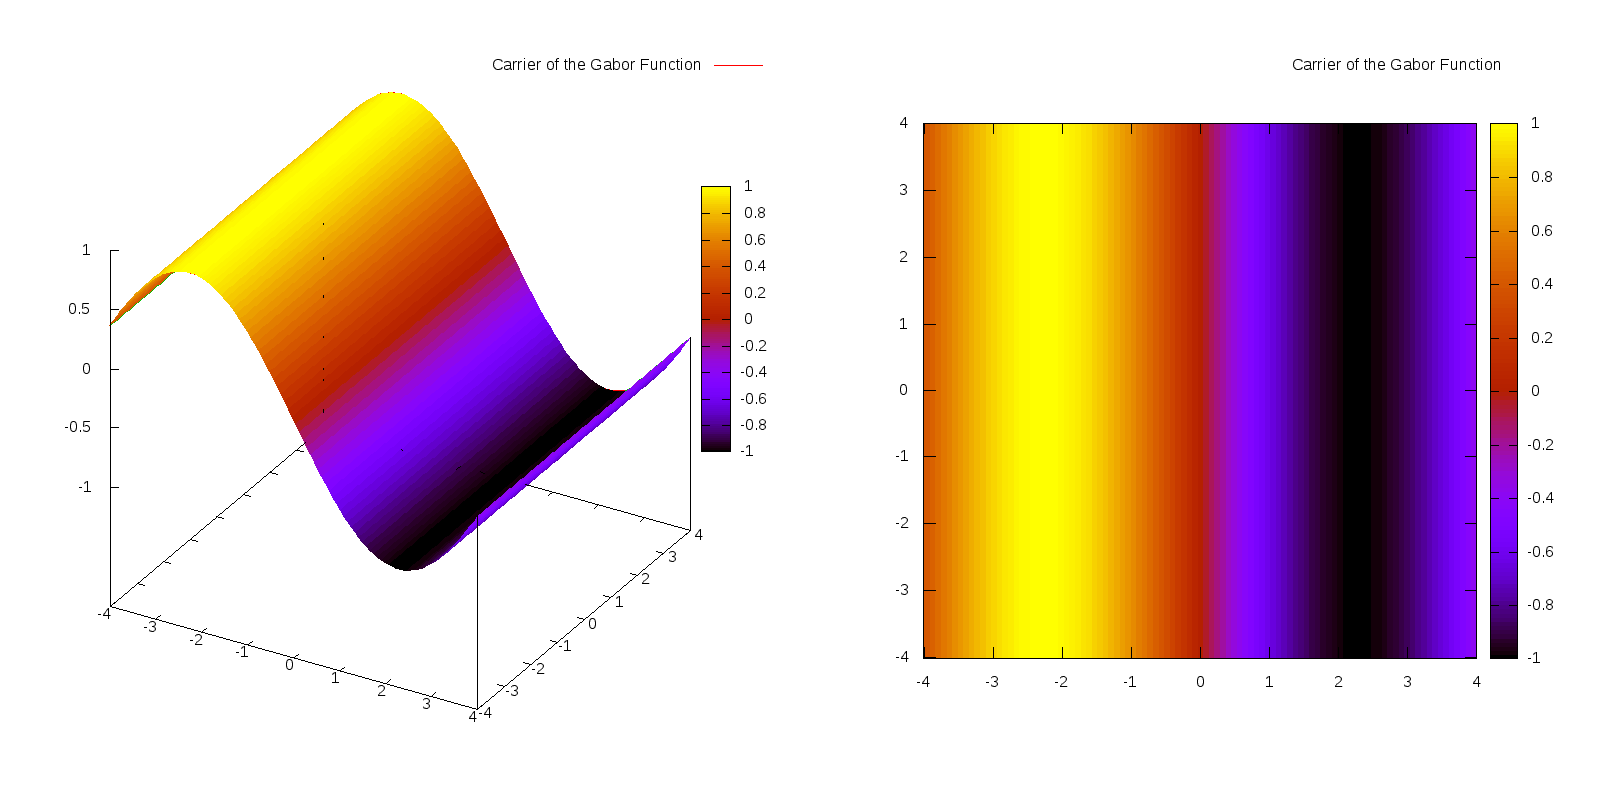
\includegraphics[width=1\textwidth]{images/carrier.png}
	\caption{Nośnik, element funkcji Gabora, przedstawiony w przestrzeni i jako mapa.}
	\label{fig:aGabor_carrier}
\end{figure}

\subsubsection{Powłoka}
\label{aGabor_envelope}

Powłoka, która jest twójwymiarowym odpowiednikiem funkcji Gausa ma postać, przedstawioną we wzorze \ref{eqn:aGabor_env}.

\begin{align}\label{eqn:aGabor_env}
W_r(x, y) = K \ exp(-\pi (a^2(x-x_0)^2_r + b^2(y-y_0)^2_r))
\end{align}
Gdzie: 
\begin{description}
\item [$(x_0, y_0)$] -- to szczyt funkcji
\item [$a$ i $b$] -- parametry odpowiedzialne za skalę powłoki w funkcji Gabora
\end{description}
Przedstawiony w powyższym wzorze \ref{eqn:aGabor_env} indeks dolny $_r$ odpowiada za rotację całej powłoki. Odpowiadające nawiasom z indeksem $_r$ wzory przedstawione są poniżej.
\begin{align}\label{eqn:aGabor_env__r}
(x-x_0)_r &= (x-x_0)\cos \theta + (y-y_0)\sin \theta\\
(y-y_0)_r &= -(x-x_0)\sin \theta + (y-y_0)\cos \theta
\end{align}

W efekcie czego można uzyskać powłokę przedstawioną na rysunku \ref{fig:aGabor_envelope}.

\begin{figure}[ht]
	\centering
	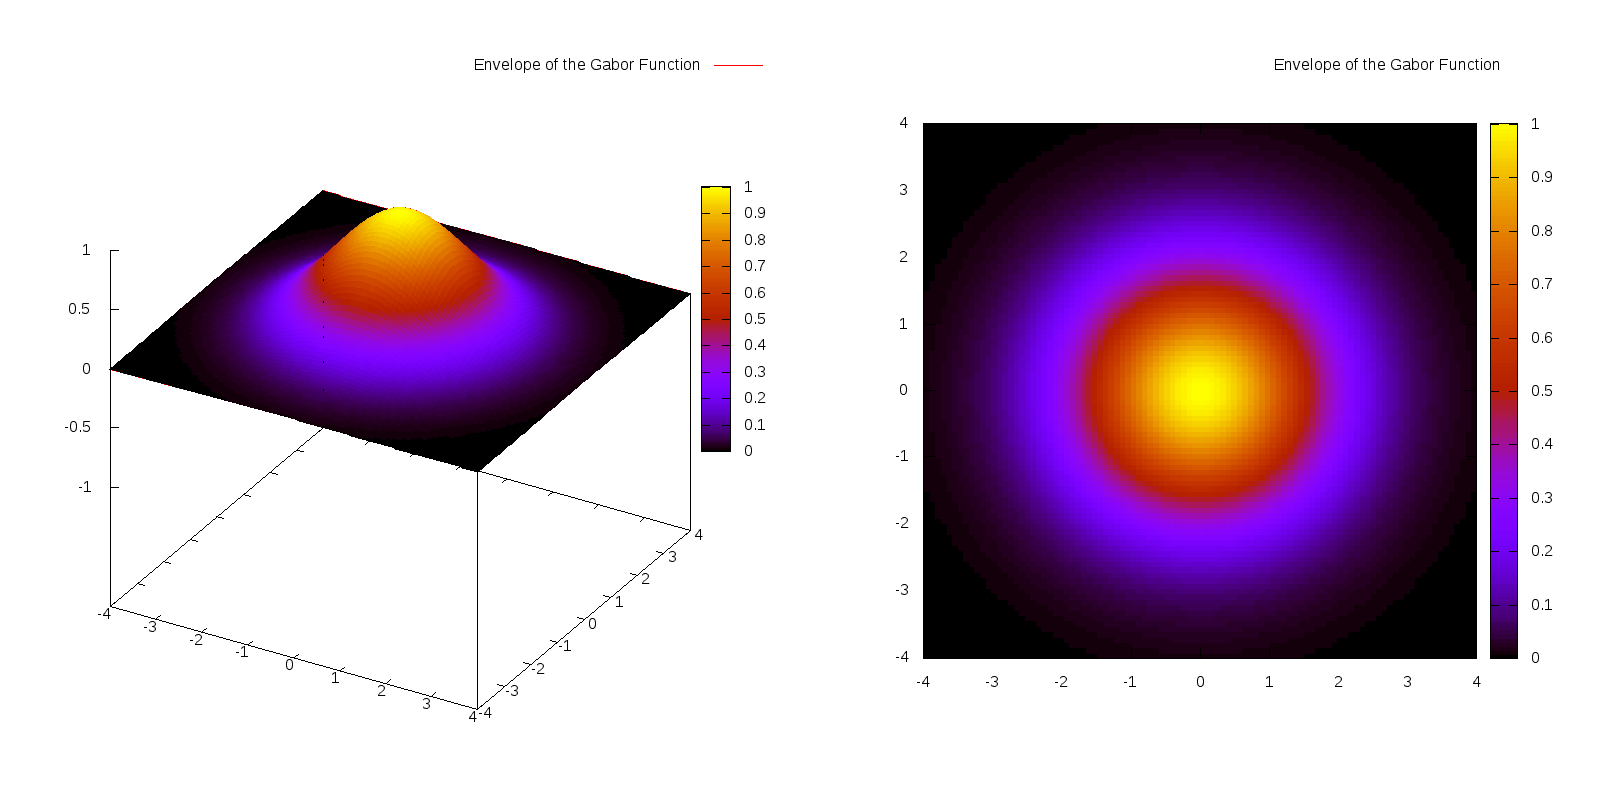
\includegraphics[width=1\textwidth]{images/envelope.png}
	\caption{Powłoka, element funkcji Gabora, przedstawiony w przestrzeni i jako mapa.}
	\label{fig:aGabor_envelope}
\end{figure}

\subsubsection{Złożenie nośnika i powłoki}
\label{aGabor_zlozenie}

\begin{figure}[ht]
	\centering
	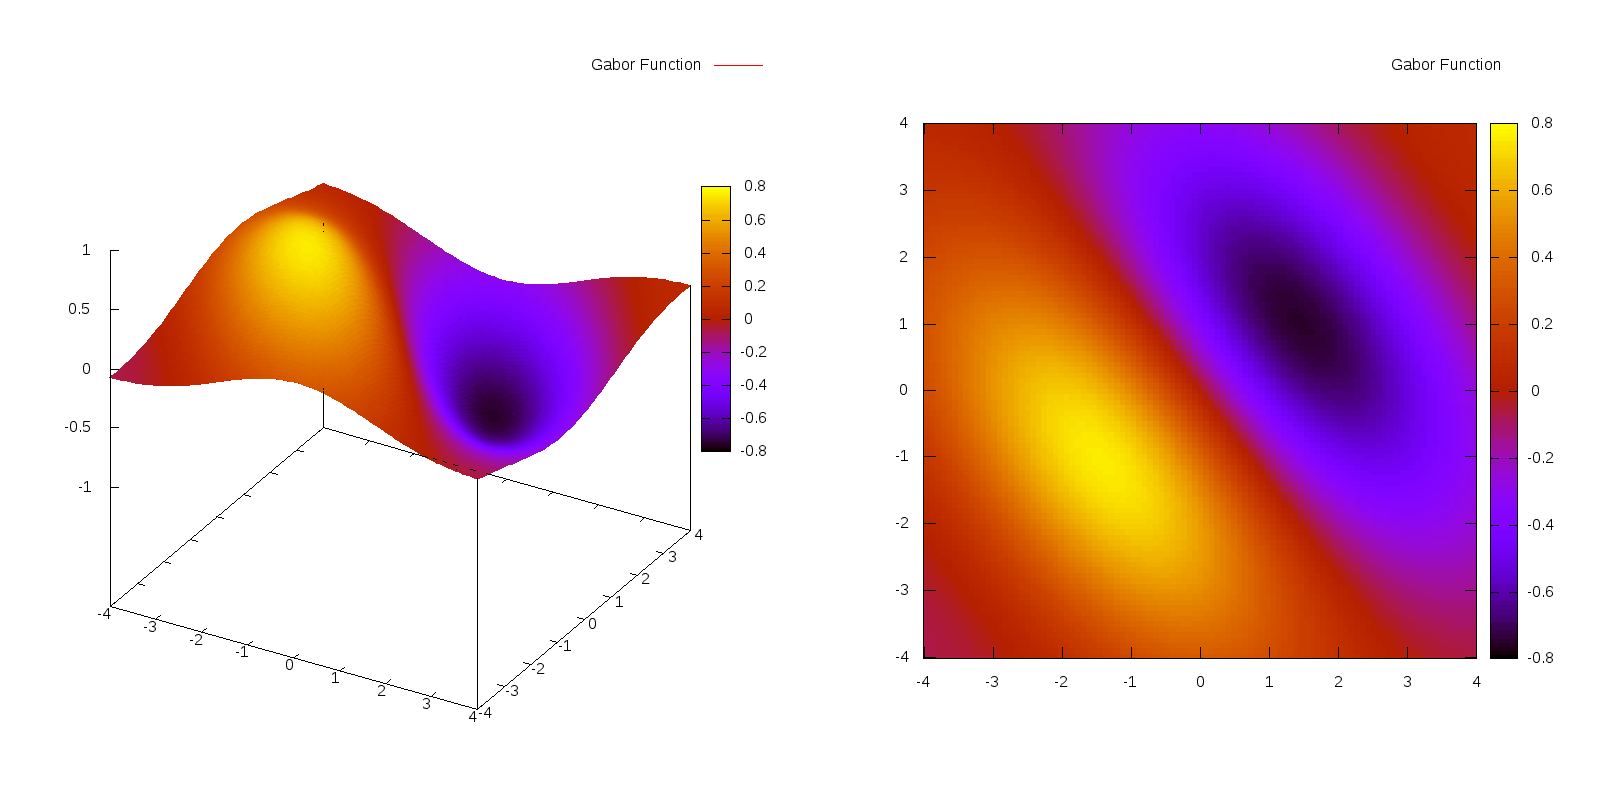
\includegraphics[width=1\textwidth]{images/gaborFunction.png}
	\caption{Funkcja Gabora przedstawiona w przestrzeni i jako mapa.}
	\label{fig:aGabor_function_res}
\end{figure}

Składając opisane wyżej funkcje ze sobą -- tak jak to jest przedstawione we wzorze \ref{eqn:aGabor_wzor1} -- można otrzymać funkcje podobne do tej, przedstawionej na rysunku \ref{fig:aGabor_function_res}.

\subsection{Filtr Gabora}
\label{aGabor_filtr}

Filtr Gabora jest połączeniem dwóch wymienionych już wcześniej technik, z taką różnicą, że jako okno filtru będzie w nim występować odpowiednio przeskalowana funkcja Gabora. Zgodnie z przedstawionym na samym początku opisem można wyprowadzić algorytm, za pomocą którego będzie można wykonać filtrowanie obrazu. Proste filtrowanie obrazu przedstawione jest w algorytmie \ref{alg:filtering}. \\

\begin{algorithm}
\caption{Zastosowanie dwuwymiarowego filtru w przetwarzaniu obrazów.}
\label{alg:filtering}
\input{algorithms/filter.algorithm}
\end{algorithm}

Filtrowanie przedstawione w algorytmie \ref{alg:filtering} pokazuje samą zasadę działania wszystkich filtrów w grafice komputerowej. Algorytm zakłada, że macierz filtru -- określana na początku załącznika jako okno filtru -- jest prostokątem, którego boki są dowolną liczbą naturalną nieparzystą. Jest to warunek, w który powoduje, że łatwiej jest sobie wyobrazić sposób działania filtru i jego sens. Dodatkowo należy wspomnieć, że zaprezentowany algorytm nie uwzględnia sytuacji w których dla piksla będącego na krawędzi w obrazie źródłowym, wyliczana jest suma ważona wraz z pikslami, które są poza obrazem. Rzecz jasna jest to sytuacja niedopuszczalna i problem należałoby rozwiązać sprawdzając, w kroku \texttt{11} czy piksel z otoczenia istnieje w obrazie źródłowym. Ostatnia modyfikacja, jaka powinna zostać przeprowadzona na algorytmie polega na zachowaniu zakresu wartości kolorów w pikslach. Wymagane jest choćby zastosowanie transformacji z ostatniego akapitu części \ref{aGabor_teoria}.\\

\begin{figure}[ht]
	\centering
	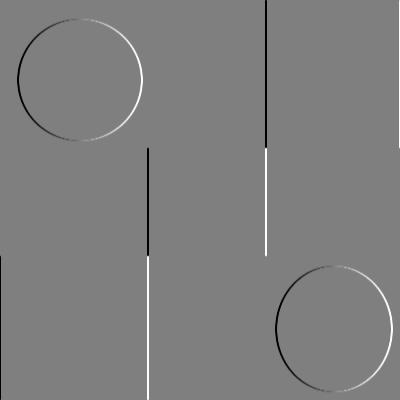
\includegraphics[width=0.3\textwidth]{images/filtering_example/simple.png}
	\caption{Wynik filtrowania obrazu \ref{fig:GF_output_input} pierwotną wersją filtru Gabora.}
	\label{fig:aGabor_simple_filter_result}
\end{figure}

Dodatkowo można zauważyć pewną prawidłowość podczas filtrowania obrazów, która jest istotna ze względów stricte wydajnościowych. O ile bowiem samego procesu filtrowania pojedynczego obrazu nie można przyśpieszyć, to filtrowanie obrazu mające na celu wyodrębnienie krawędzi filtrem Gabora -- przedstawiane w obrazach \ref{fig:GF_output}b-k -- można dwukrotnie przyspieszyć. Należy bowiem zwrócić uwagę na to, że filtrując obraz (choćby \ref{fig:GF_output_input}) filtr będzie w wynikowym obrazie ciemniejsze kolory dawać krawędziom występującym w okolicach piksli, których suma ważona będzie największa. Patrząc na krok \texttt{11} algorytmu \ref{alg:filtering} widać, że wagi do tej sumy są umieszczone w oknie filtru, przez co maksymalna wartość będzie przypadać na piksel, w którego otoczeniu piksle będą tak ułożone, że minusy przy iloczynie się skrócą. I w pierwotnej wersji algorytmu jedynie o to chodziło. Zwracając jednak uwagę na zaistniały fakt można by powiedzieć, że odwrotna sytuacja zostanie zaobserwowana gdy filtrowaniu obrazu poddany zostanie fragment obrazu, w którym krawędź jest odwrotna, w sensie minusy przy iloczynie się nie skrócą a piksel otrzyma minimalną wartość. Obrazek przedstawiający zaistniałą sytuację przedstawiony jest na rysunku \ref{fig:aGabor_simple_filter_result}. Aby takie sytuacje wyeliminować, można zastosować niewielkie uproszczenie kodu z algorytmu \ref{alg:filtering} w którym w kroku \texttt{14} będzie wykonywać dodatkowe sprawdzenie, takie jak to, przedstawione w algorytmie \ref{alg:filteringspeedup}. Dzięki czemu będzie można otrzymywać rezultaty podobne do tych z rysunku \ref{fig:GF_output}.

\begin{algorithm}
\caption{Modyfikacja kroku 14 algorytmu \ref{alg:filtering}.}
\label{alg:filteringspeedup}
\input{algorithms/filterspeedup.algorithm}
\end{algorithm}


\subsection{Przykład filtrowania}
\label{aGabor_przyklad}

Filtrowanie z zastosowaniem zmodyfikowanego algorytmu \ref{alg:filtering} na obrazie monochromatycznym daje ciekawe rezultaty, jak pokazuje rysunek \ref{fig:GF_output}.

\begin{figure}[ht]
  \centering
  \subfloat[Obraz wejściowy]{\label{fig:GF_output_input}
\includegraphics[width=0.3\textwidth]{images/filtering_example/one.png}}               
  \subfloat[$\omega_0 = 0$]{\label{fig:GF_output_w00}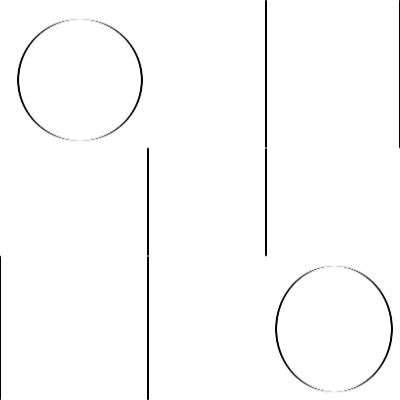
\includegraphics[width=0.3\textwidth]{images/filtering_example/000.png}}
  \subfloat[$\omega_0 = 0.1$]{\label{fig:GF_output_w01}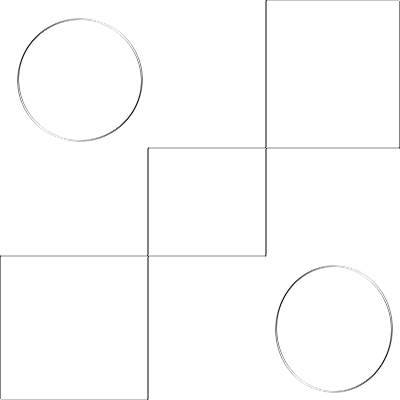
\includegraphics[width=0.3\textwidth]{images/filtering_example/001.png}}\\
  \subfloat[$\omega_0 = 0.2$]{\label{fig:GF_output_w02}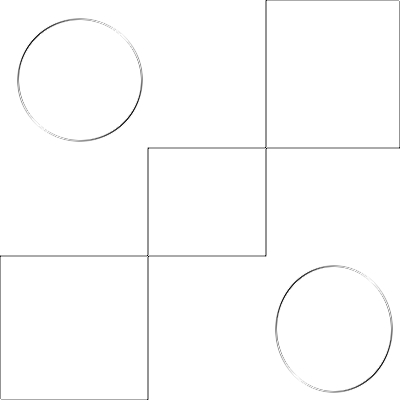
\includegraphics[width=0.3\textwidth]{images/filtering_example/002.png}}
  \subfloat[$\omega_0 = 0.3$]{\label{fig:GF_output_w03}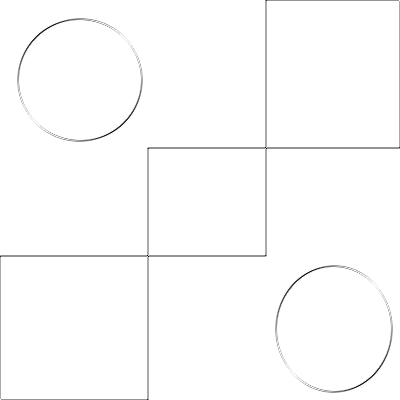
\includegraphics[width=0.3\textwidth]{images/filtering_example/003.png}}
  \subfloat[$\omega_0 = 0.4$]{\label{fig:GF_output_w04}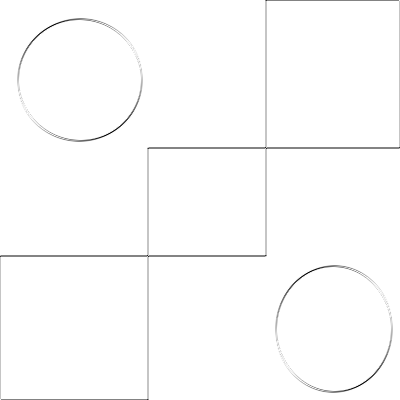
\includegraphics[width=0.3\textwidth]{images/filtering_example/004.png}}\\
  \subfloat[$\omega_0 = 0.5$]{\label{fig:GF_output_w05}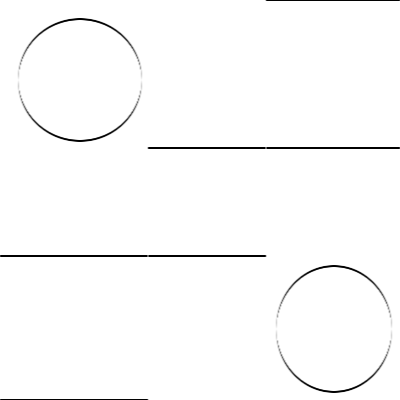
\includegraphics[width=0.3\textwidth]{images/filtering_example/005.png}}
  \subfloat[$\omega_0 = 0.6$]{\label{fig:GF_output_w06}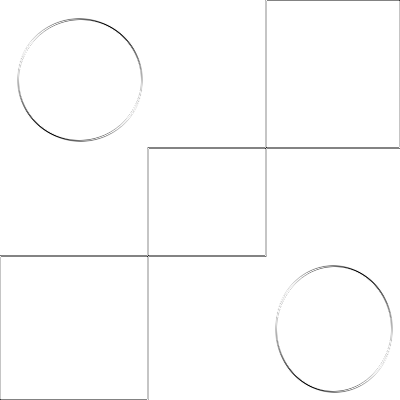
\includegraphics[width=0.3\textwidth]{images/filtering_example/006.png}}
  \subfloat[$\omega_0 = 0.7$]{\label{fig:GF_output_w07}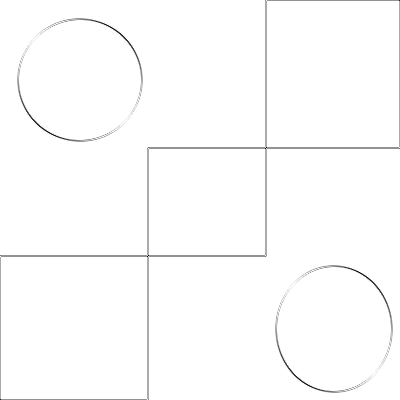
\includegraphics[width=0.3\textwidth]{images/filtering_example/007.png}}\\
  \subfloat[$\omega_0 = 0.8$]{\label{fig:GF_output_w08}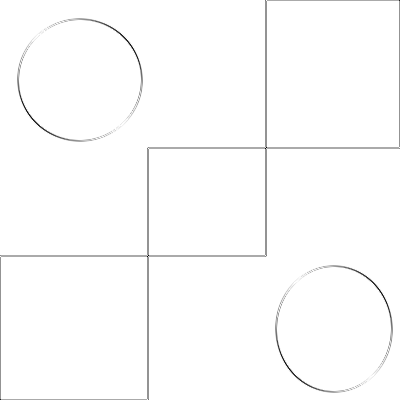
\includegraphics[width=0.3\textwidth]{images/filtering_example/008.png}}
  \subfloat[$\omega_0 = 0.9$]{\label{fig:GF_output_w09}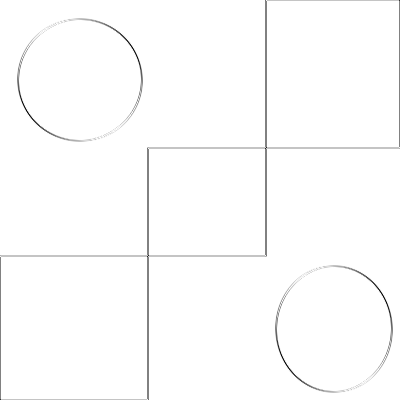
\includegraphics[width=0.3\textwidth]{images/filtering_example/009.png}}
  \caption{Wyniki filtrowania obrazu \ref{fig:GF_output_input} filtrami Gabora w których $\omega_0$ jest w przedziale $(0, 1>$.}
  \label{fig:GF_output}
\end{figure}

Co warto nadmienić, filtr Gabora przy jednokrotnym zastosowaniu nie wykryje wszystkich krawędzi w obrazie. Jak można zobaczyć na obrazie \ref{fig:GF_output}b-k przy konkretnej wartości kąta $\omega_0$ wyraźniejsze są konkretne krawędzie. Istotne jest więc wyodrębnienie krawędzi pod wszystkimi kątami (z dowolną dokładnością) i połączenie obrazów w taki sposób, że dla każdego konkretnego piksla w obrazie brane będzie maksymalne nasycenie koloru z wszystkich obrazów składowych.\\

Rysunek \ref{fig:GF_output_join} przedstawia obraz wejściowy i wynik etapu filtrowania, na którym bardzo dobrze są widoczne krawędzie obrazu.

\begin{figure}[ht]
  \centering
  \subfloat[Obraz wejściowy]{\label{fig:GF_output_input2}
\includegraphics[width=0.3\textwidth]{images/filtering_example/one.png}}               
  \subfloat[Otrzymany wynik]{\label{fig:GF_output_join2}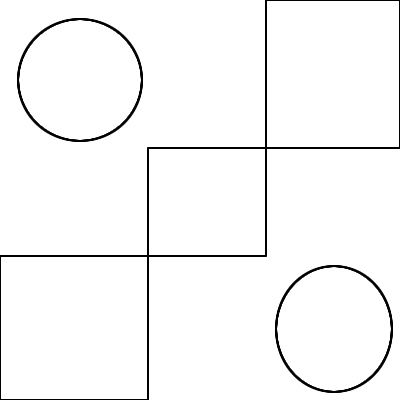
\includegraphics[width=0.3\textwidth]{images/filtering_example/join.png}}
  \caption{Wyniki filtrowania obrazu \ref{fig:GF_output_input2} filtrami Gabora oraz operacji połączenia otrzymywanych rezultatów w jeden obraz.}
  \label{fig:GF_output_join}
\end{figure}

\section{Dyskusja i wnioski}
\label{aGabor_dyskusja}

Wyniki pracy zaprezentowane w poprzednich etapach świadczą o skuteczności zaznaczania krawędzi w obrazach. Co było już podkreślane w pierwszych częściach tego dokumentu -- nie tylko Gabor wpadł na dobry pomysł, natura sama od ,,zawsze'' stosuje coś podobnego w korze wzrokowej \cite{Jones1987}. Ale co należy podkreślić, sam filtr Gabora nie jest skutecznym rozwiązaniem. Przedstawione poniżej, na rysunku \ref{fig:GF_compare} obrazki a-f pokazują, że istotny jest preprocessing\footnote{Zapożyczone z języka angielskiego -- wstępne przetworzenie.} obrazów, aby zmniejszyć liczbę występujących w obrazie zakłóceń. Dodatkowo widać, że nie tylko kąt funkcji sinus -- będącej składową filtru Gabora -- jest istotny, ale również wielkość okna filtru. Mimo, że obrazy są tendencyjne pod względem prezentacji szczegółowych obiektów, na których widać wyraźne krawędzie, można sobie wyobrazić jednak obrazy z mniej wyraźnymi krawędziami, na których większe okno lepiej by sobie radziło.

\begin{figure}[ht]
  \centering
  \subfloat[Obraz wejściowy]{\label{fig:GF_compare_in_1}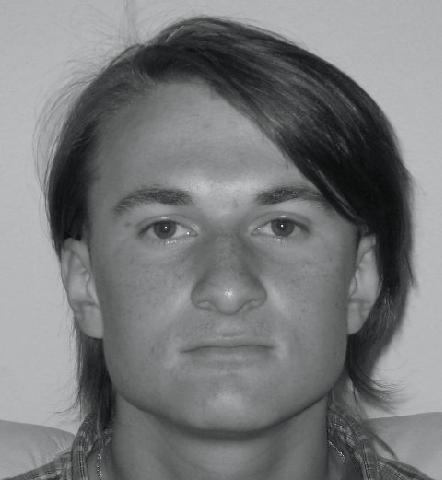
\includegraphics[width=0.3\textwidth]{images/filtering_example/asdf.JPG}}               
  \subfloat[Filtracja oknem $3\times3$]{\label{fig:GF_compare_1_f3}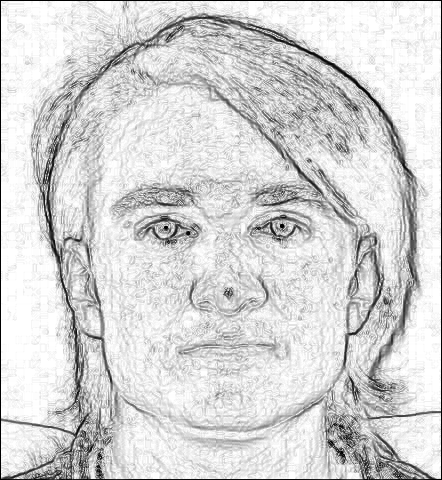
\includegraphics[width=0.3\textwidth]{images/filtering_example/100.png}}
  \subfloat[Filtracja oknem $9\times9$]{\label{fig:GF_compare_1_f9}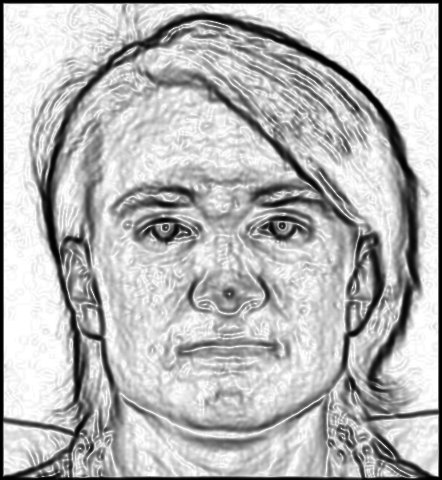
\includegraphics[width=0.3\textwidth]{images/filtering_example/102.png}}\\
  \subfloat[Obraz wejściowy wstępnie przetworzony]{\label{fig:GF_compare_in_2}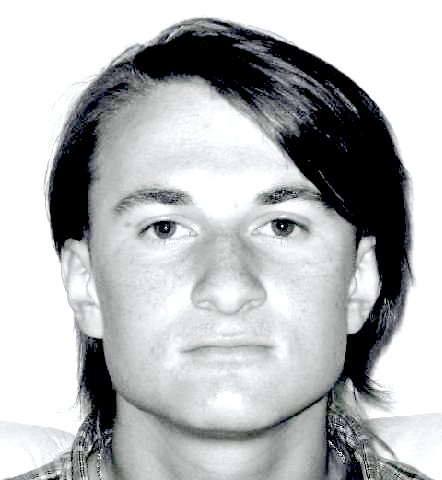
\includegraphics[width=0.3\textwidth]{images/filtering_example/myself2.JPG}}
  \subfloat[Filtracja oknem $3\times3$]{\label{fig:GF_compare_2_f3}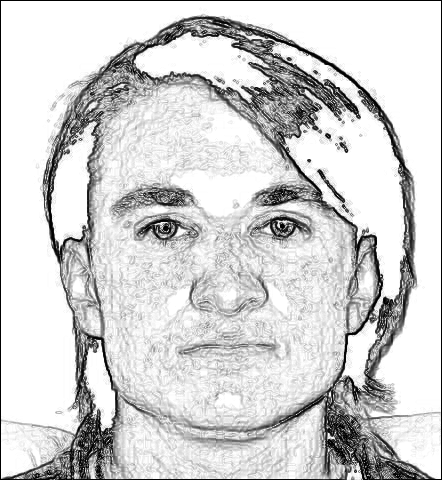
\includegraphics[width=0.3\textwidth]{images/filtering_example/101.png}}
  \subfloat[Filtracja oknem $9\times9$]{\label{fig:GF_compare_2_f9}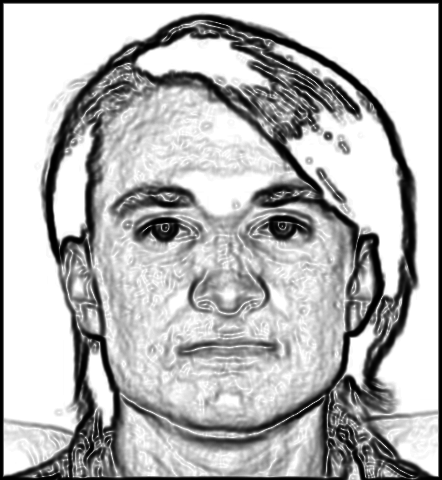
\includegraphics[width=0.3\textwidth]{images/filtering_example/103.png}}
  \caption{Wyniki filtrowania obrazów \ref{fig:GF_compare_in_1} i \ref{fig:GF_compare_in_2} filtrami Gabora w których różna była wielkość okna filtru.}
  \label{fig:GF_compare}
\end{figure}

Co widać teraz wyraźnie na przedstawianych obrazach, to fakt, że wyraźne oprócz środkowych części obrazu są też krawędzie. Dla nich bowiem proces filtrowania nie mógł być przeprowadzony z uwagi na brak sąsiednich piksli, które były by brane spoza obrazu. Przy dalszym przetwarzaniu obrazów wypadałoby tych krawędzi nie brać pod uwagę.

